%-------------------------------------------------------------------------------
\section{Design}
%-------------------------------------------------------------------------------

\begin{figure*}[ht!]
    \centering
    \begin{subfigure}[t]{0.5\textwidth}
        \centering
        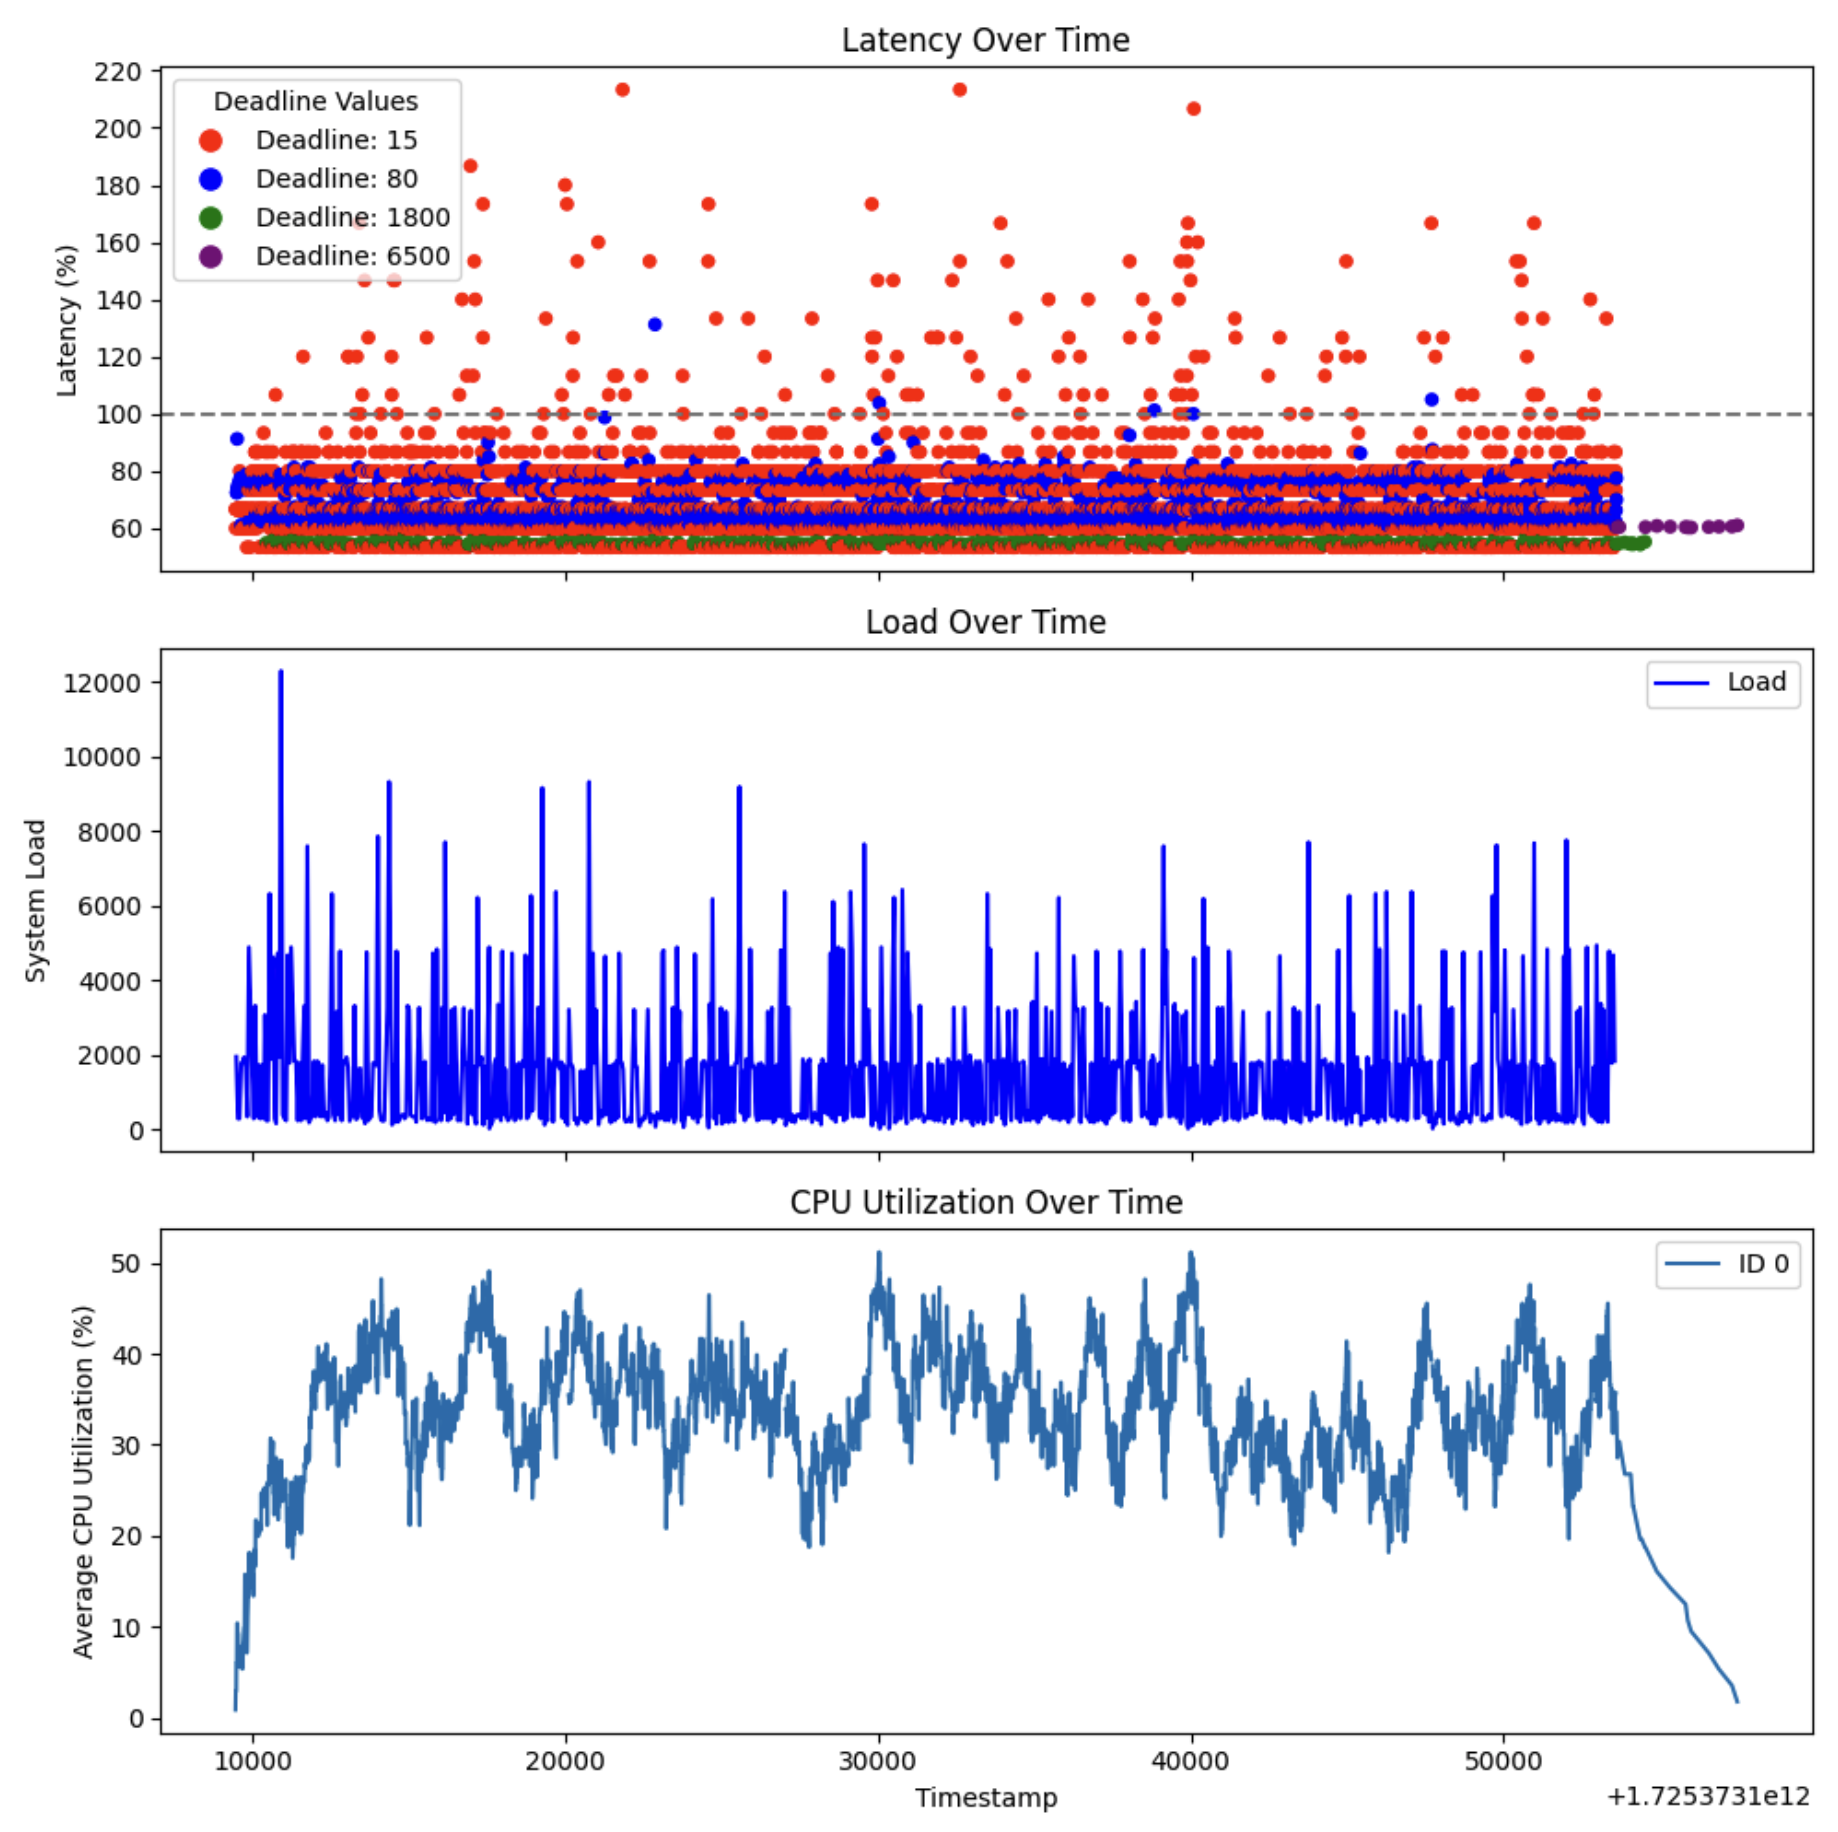
\includegraphics[height=1.2in]{img/old_lnx__2ms_wait__10K_iter.png}
        \caption{Latency and load in original linux}
    \end{subfigure}%
    \hfill
    \begin{subfigure}[t]{0.5\textwidth}
        \centering
        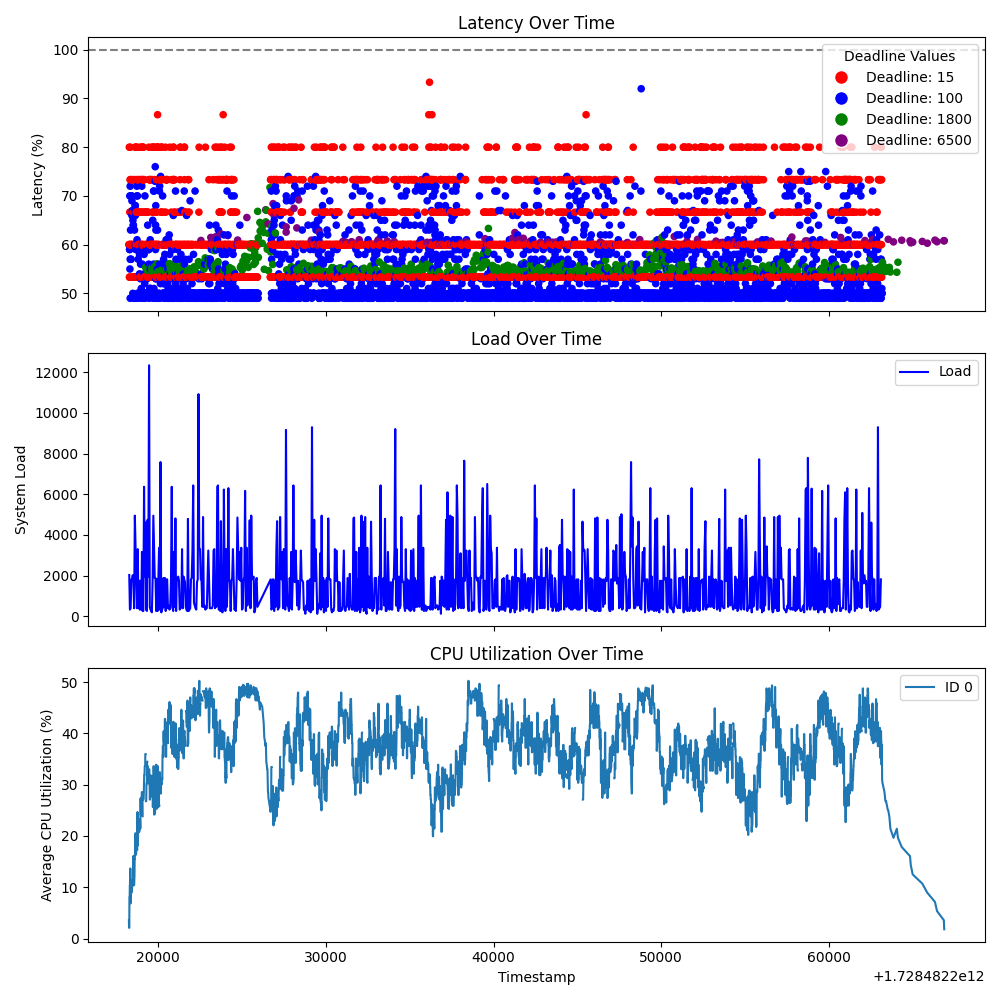
\includegraphics[height=1.2in]{img/new_lnx__2ms_wait__10K_iter.png}
        \caption{Latency and load in modified linux}
        \label{fig:graph:new}
    \end{subfigure}
    \vspace{10pt}
    \caption{Results of running the same workload on (a) unmodified and (b) modified linux.}
    \label{fig:graph}
\end{figure*}

When a job needs to be run, \sysname{} initially routes it to the relevant shard
of the global scheduler, which then forwards the job to a chosen single machine.


\subsection*{Distributed Global Scheduler}

Each global scheduler shard has a set of machines that it can run jobs on. The
goal of the global scheduler is to keep load as evenly distributed among these
machines as possible, in the sense that each machine has a maximally
heterogenous set of deadlines and computes. This allows processes with more
\textit{slack} (difference between deadline and max compute) to fill in gaps
where shorter processes might have finished earlier than expected (similarly to
how best effort work now opportunistically uses resources not currently used by
latency critical tasks).

Depending on the amount of slack the global scheduler will either immediately
place the job, or will probe a dynamic number of machines in order to find a
good match.


\subsection*{Single machine}

On the individual machines, the goal is to to meet all the deadlines of the work
assigned to the machine. This has two parts: one is a dispatcher thread, which
handles communication with its global scheduler shard and does admission
control; and the other is a local scheduler that prioritizes work by deadline.

\sysname{}'s admission control is pessimistic, and assumes that every process
will use the maximum compute time. The dispatcher looks at the amount of slack
each process has (given the original slack and how much time it has already
spent waiting), and judges whether with the new process it could still meet all
the maximum compute guarantees.


The local scheduler approximates Earliest Deadline First (EDF) scheduling.
\sysname{} acheives EDF scheduling by using Earliest Eligible Virtual Deadline
First (EEVDF)~\cite{eevdf} --- originally proposed in the 90s and recently
integrated in linux~\cite{linuxeevdf}.

In EEVDF, processes make requests for resources, and each request is assigned an
eligible time and a deadline. At every scheduling point, of the eligible
processes the one with the earliest deadline is chosen to run next. Eligible
times and deadlines are in virtual time, which allows for oversubscription. 

\begin{figure}[t!]
    \centering
    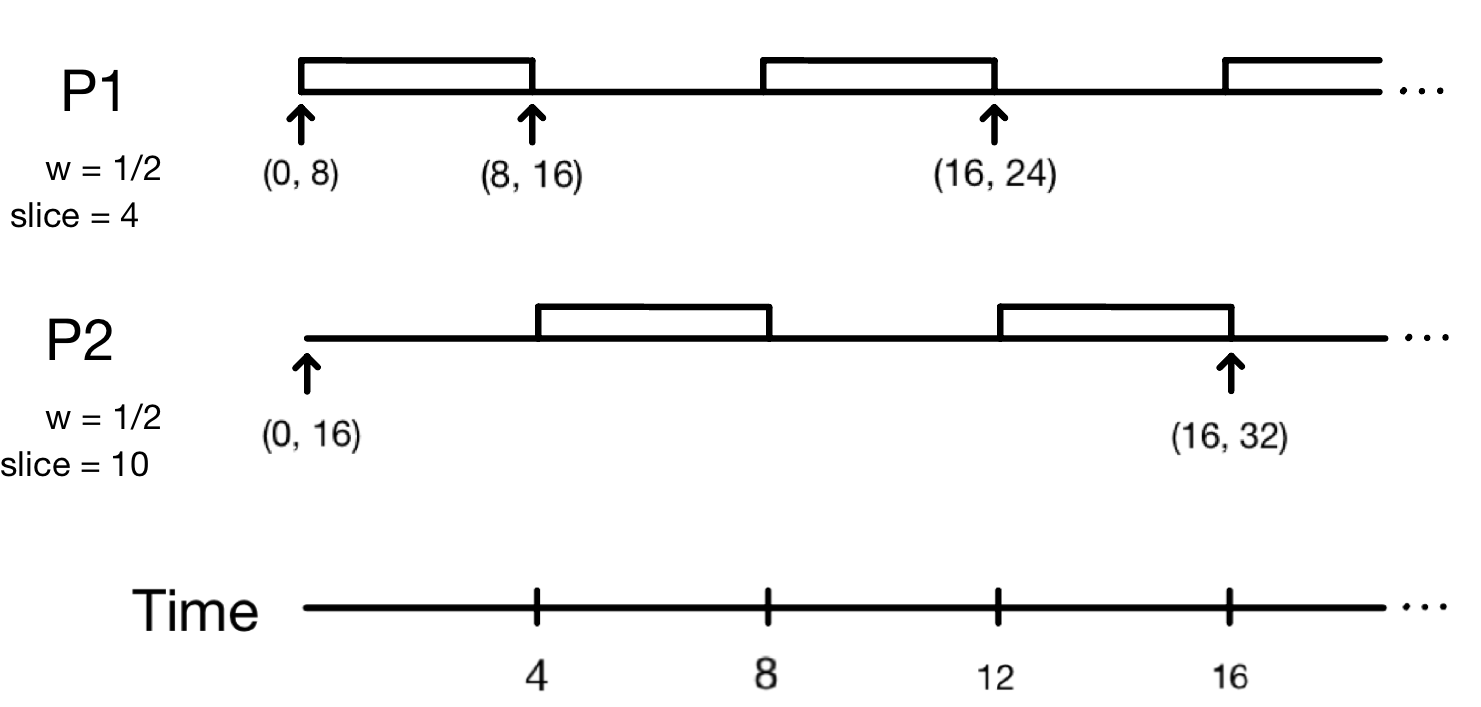
\includegraphics[height=1in]{img/eevdf.png}
    \caption{An example EEVDF timeline. Arrows represent requests, denoted with
        time eligible and deadline, and boxes show which process was chosen to
        run.}
    \label{fig:eevdf}
\end{figure}

Processes need to be able to be ineligible in order to maintain fairness. If a
process ran for the last tick and completed its latest request, its next
eligible time will be set to be in the future (a weighted estimation of by when
it should have gotten the time it just did, based on its weight as well the the
total system load). This protects against starvation of processes with longer
deadlines. Figure~\ref{fig:eevdf} shows a scheduling flow for two equally weighted
processes.

If jobs make requests often and for small time increments, this policy is
similar to Process Sharing (PS) --- each process runs for a scheduling quanta
before becoming ineligible. However, on the other extreme you get behavior
closer to EDF --- if jobs only ever make one request for all the resources that
they think they will need, then the requests never reset and all processes are
always elgibible. Since the EEVDF scheduler is by definition choosing the
eligible process with the earliest deadline (and all processes are always
eligible), it is effectively implementing EDF.

And creating this edge condiiton is what the dispatcher does --- when it spawns
a process for a new job, it sets the requested timeslice of that job to be the
jobs maximum compute. 

